\section{PRELIMINARIES}
\label{sec:PRELIMINARIES}
This paper designs   SRLG disjoint routing algorithm based on the max-flow min-cut theorem. This section introduces the preliminaries on the theorem.
\subsection{Maximum flow}
Let $G=(\mathbb{\mathbb{V}},\mathbb{\mathbb{E}})$ be a network (where $\mathbb{\mathbb{V}}$ is the set of $|\mathbb{\mathbb{V}}|$ nodes  and $\mathbb{\mathbb{E}}$ is the set of $|\mathbb{\mathbb{E}}|$ links) with $s\in \mathbb{V}$ and $d\in \mathbb{V}$ being the source and the destination respectively.

The \textbf{capacity} of  link $e_i$, denoted by $c_{e_i}$, represents the maximum amount of flow that can pass through the link. A \textbf{flow}  of  link, denoted by $f_{e_i}$, should meet the following two constraints:

1) Capacity Constraint: $\forall e_i\in \mathbb{\mathbb{E}}$: $f_{e_i}\leq c_{e_i}$.

2) Conservation of Flows: $\forall u\in \mathbb{\mathbb{V}}-\{s,d\}$: $\sum\limits_{v\in \mathbb{V}}f_{(v,u)}=\sum\limits_{v\in \mathbb{V}}f_{(u,v)}$, where $(v,u)$ and $(u,v)$ denote the links $e(v,u)$ and $e(u,v)$.

The \textbf{value of flow} is defined by $|f|=\sum\limits_{v\in \mathbb{V}}f_{(s,v)}$, where $s$ is the source. It represents the amount of flow passing from   $s$ to   $d$.

\textbf{Maximum Flow Problem}: The goal is to maximize $|f|$ by routing as much flow as possible from $s$ to $d$.
\subsection{Minimum cut}
An \textbf{s-d cut} ${\Phi}=(\mathbb{S},\mathbb{D})$  is a partition of $\mathbb{V}$ such that $s \in \mathbb{S}$ and $d \in \mathbb{D}$. The \textbf{cut-set} $\mathbb{\mathbb{L}}_{\Phi}$ of $\Phi$ is the link set
\begin{equation}
\mathbb{\mathbb{L}}_{\Phi}=\{(u,v)\in \mathbb{E}: u \in \mathbb{S}, v \in \mathbb{D}\}.
\end{equation}
Note that if the links in the cut-set $\mathbb{\mathbb{L}}_{\Phi}$ are removed, then $|f| = 0$. That is, no flow can pass from $s$ to $d$. In this paper,  we try to find the SRLG Conflicting Link Set based on the feature of the cut-set.

The capacity of an s-d cut $\Phi$ is defined by $c(\Phi)=\sum\limits_{e_i\in \mathbb{\mathbb{L}}_{\Phi}}c_{e_i}$.

\textbf{Minimum s-d Cut $\Phi$ Problem}: Minimize $c(\Phi)$, that is, to determine $\mathbb{S}$ and $\mathbb{D}$ such that the capacity ($c(\Phi)$) of the s-d cut ${\Phi}=(\mathbb{S},\mathbb{D})$ is minimal.




\subsection{Max-flow min-cut theorem}
\textbf{Max-flow min-cut theorem}: The maximum value of an $s-d$ flow is equal to the minimum capacity over all $s-d$ cuts.
\begin{figure}[tp]
  \centering
  % Requires \usepackage{graphicx}
  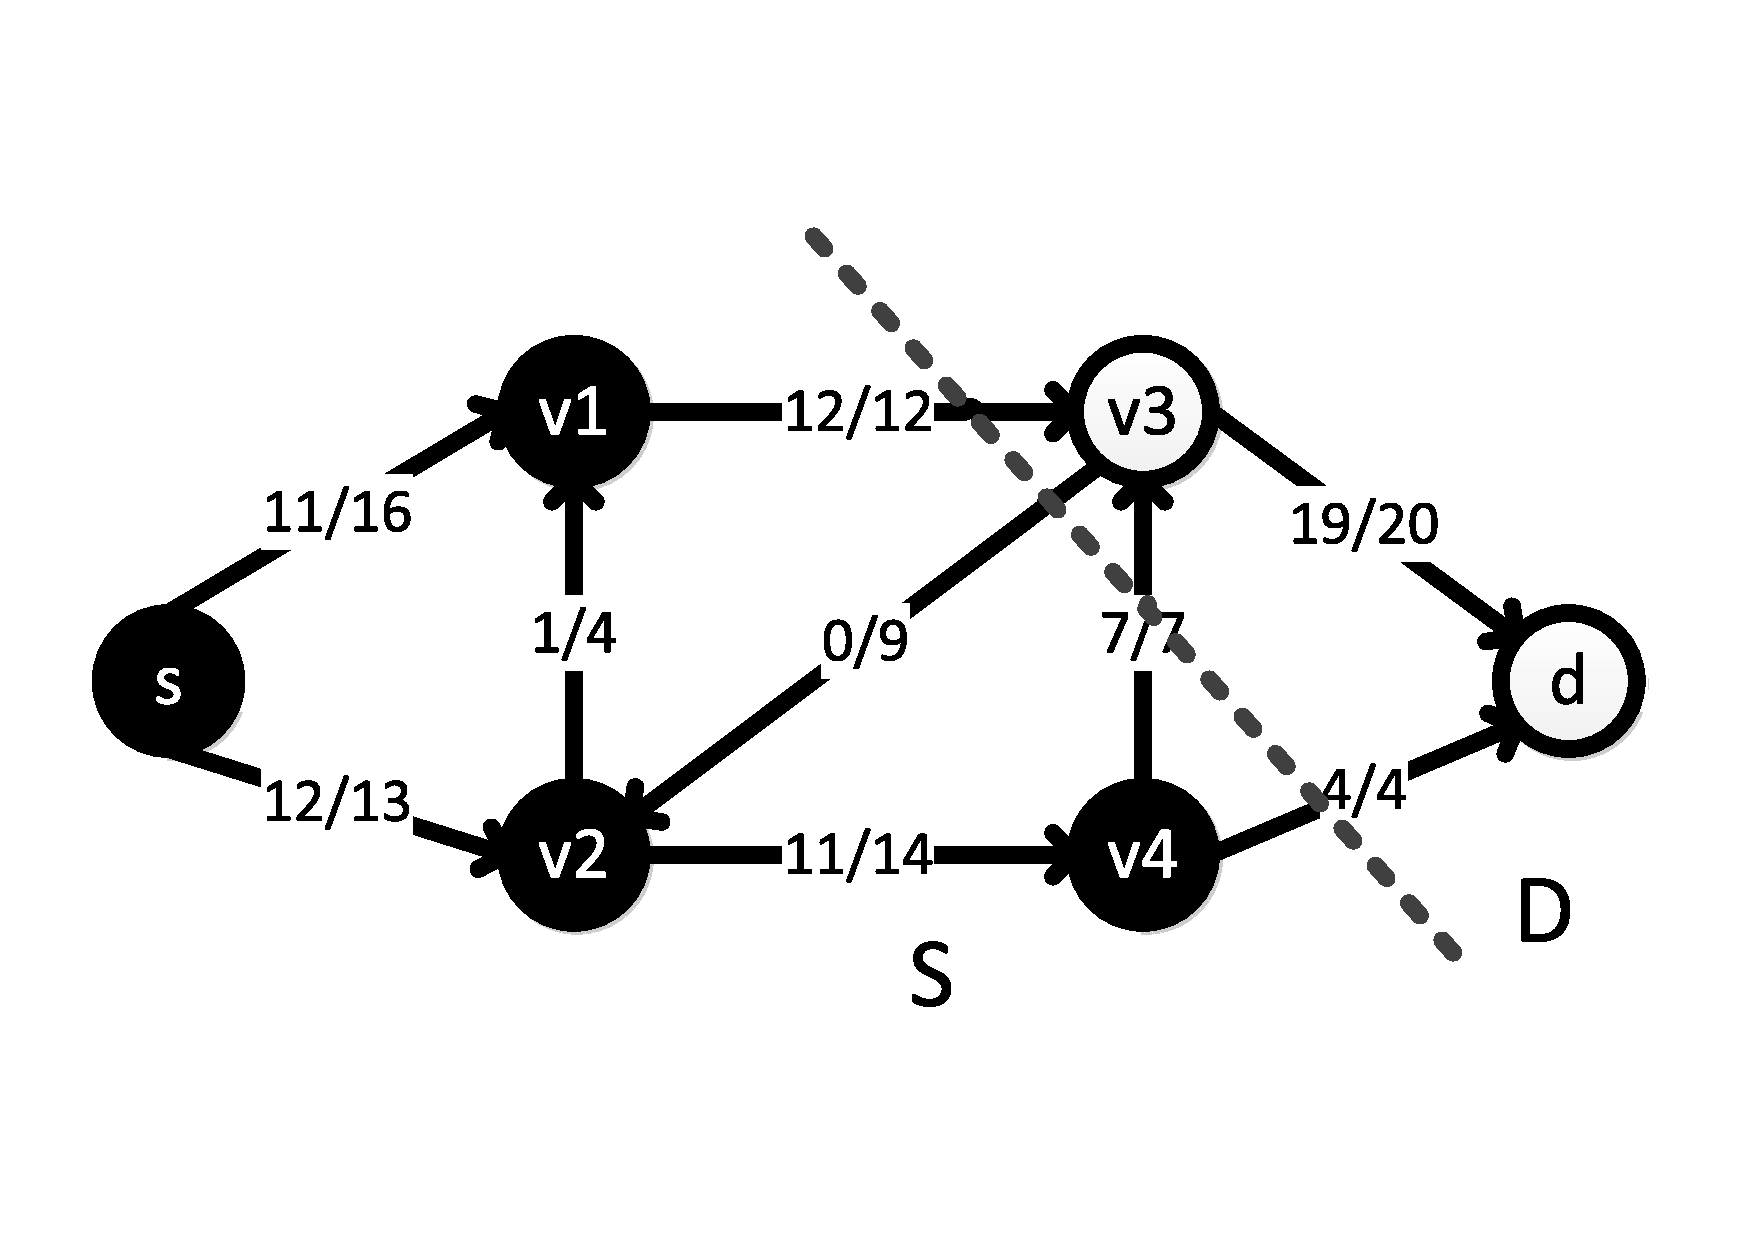
\includegraphics[width=2.5in]{franz//FlowNetwork}\\
  \caption{An example to illustrate max-flow min-cut theorem. Each link $e_i$ is labeled by $f_{e_i}/c_{e_i}$, where $f_{e_i}$ and $c_{e_i}$ denote the flow and capacity of link $e_i$, respectively.   }
  \label{fig:FlowNetwork}
\end{figure}
In Fig.\ref{fig:FlowNetwork}, max-flow $f$ in $G$ with its value $|f|=f_{(s,v_1)}+f_{(s,v_2)}$. The cut $\Phi(\mathbb{S},\mathbb{D})$ with $\mathbb{S}=\{s,v_1,v_2,v_4\}$ and $\mathbb{D}=\{v_3,d\}$ is the min-cut with its capacity $c(\Phi)=c_{(v_1,v_3)}+c_{(v_4,v_3)}+c_{(v_4,d)}=12+7+4=23$. Obviously, $|f|=c(\Phi)$, that is, the maximum value of an s-d flow is equal to the minimum capacity over all s-d cuts.

%
%We are now ready to define flows more formally. Let $G=(\mathbb{V},\mathbb{E})$ be a flow network in which each link $(u,v)\in \mathbb{E}$ has a nonnegative capacity $c(u,v)\geq 0$. Let s be the source of the network, and let $d$ be the sink. A flow in $G$ is a real-valued function $f:\mathbb{V}\times \mathbb{V} \rightarrow {\mathbb{R}}$ that satisfies the following two properties:
%\begin{itemize}
%  \item Capacity constraint: For all $u,v\in \mathbb{V}$, we require $0\leq f(u,v)\leq c(u,v)$.
%  \item Flow conservation: For all $u\in \mathbb{V}-\{s,t\}$, we require $\sum\limits_{v\in \mathbb{V}}f(v,u)=\sum\limits_{v\in \mathbb{V}}f(u,v)$. when $(u,v)\notin \mathbb{E}$, there can be no flow from $u$ to $v$, and $f(u,v)=0$.
%\end{itemize}
%
%We call the nonnegative quantity $f(u,v)$ the flow from vertex $u$ to vertex $v$. The value $|f|$ of a flow $f$ is defined as $|f|=\sum\limits_{v\in \mathbb{V}}f(s,v)-\sum\limits_{v\in \mathbb{V}}f(v,s)$. In the maximum-flow problem, we are given a flow network $G$ with source $s$ and sink $d$ , and we wish to find a flow $|f|$ of maximum value. Fig.\ref{fig:FlowNetwork} show an example of a flow network.


%
%\subsection{Cuts of flow networks}
%A cut $\Phi(\mathbb{S},\mathbb{D})$ of flow network $G=(\mathbb{V},\mathbb{E})$ is a partition of $\mathbb{V}$ into $\mathbb{S}$ and $\mathbb{D}=\mathbb{V}-\mathbb{S}$ such that $s\in \mathbb{S}$ and $d\in \mathbb{D}$. If $f$ is a flow, then the net flow $f(\mathbb{S},\mathbb{D})$ across the cut $(\mathbb{S},\mathbb{D})$ is defined to be $f(\mathbb{S},\mathbb{D})=\sum\limits_{u\in \mathbb{S}}\sum\limits_{v\in \mathbb{D}}f(u,v)-\sum\limits_{u\in \mathbb{S}}\sum\limits_{v\in \mathbb{D}}f(v,u)$. The capacity of the cut $\Phi(\mathbb{S},\mathbb{D})$ is $c(\mathbb{S},\mathbb{D})=\sum\limits_{u\in \mathbb{S}}\sum\limits_{v\in \mathbb{D}}c(u,v)$. A minimum cut of a network is a cut whose capacity is minimum over all cuts of the network.
%
%The asymmetry between the definition of flow and capacity of a cut is intentional and important. For capacity, we count only the capacity of links going from $\mathbb{S}$ to $\mathbb{D}$, ignoring links in the reverse direction. For flow, we consider the flow going from $\mathbb{S}$ to $\mathbb{T}$ minus the flow going in the reverse direction from $\mathbb{T}$ to $\mathbb{S}$. We call the capacitated links (links with non-zero capacity) from $\mathbb{S}$ to $\mathbb{D}$ positive links ${\mathbb{L}}$ and the capacitated links from $\mathbb{D}$ to $\mathbb{S}$ negative links ${\mathbb{T}}$. A min-cut is a $\Phi(\mathbb{S},\mathbb{D})$ cut whose positive capacity is minimal. Fig.\ref{fig:FlowNetwork} shows the cut ($\{s,v_1,v_2,v_4\},\{v_3,d\}$) in the flow network.
%
%\subsection{Max-flow min-cut theorem\cite{ford2015flows}}
%The value of any flow from $s$ to $d$ in $G$ is bounded by the positive capacity of the min-cut of $G$, $f(\mathbb{S},\mathbb{D})\leq c(\mathbb{S},\mathbb{D})$. The maximal flow $|f|$ value from $s$ to $d$ is equal to the minimum $c(\mathbb{S},\mathbb{D})_{min}$ of the capacities of cuts separating $s$ from $d$. $|f|=c(\mathbb{S},\mathbb{D})_{min}$
